% nicht vergessen draft raus zu nehmen, um echte Bilder einzubinden und die Problem-Vierecke verschwinden zu lassen
\documentclass[11pt,a4paper,oneside,svgnames]{report}

\usepackage[british]{babel}
\usepackage[utf8]{inputenc}
\usepackage[T1]{fontenc}
\usepackage{ae}
\usepackage{graphicx}
\usepackage{tikz}
\usepackage{kpfonts}
\usepackage[explicit]{titlesec}


\newcommand*\chapterlabel{}
\titleformat{\chapter}
  {\gdef\chapterlabel{}
   \normalfont\sffamily\Huge\bfseries\scshape}
  {\gdef\chapterlabel{\thechapter\ }}{0pt}
  {\begin{tikzpicture}[remember picture,overlay]
    \node[yshift=-3cm] at (current page.north west)
      {\begin{tikzpicture}[remember picture, overlay]
        \draw[fill=LightSkyBlue] (0,0) rectangle
          (\paperwidth,3cm);
        \node[anchor=east,xshift=.9\paperwidth,rectangle,
              rounded corners=20pt,inner sep=11pt,
              fill=MidnightBlue]
              {\color{white}\chapterlabel#1};
       \end{tikzpicture}
      };
   \end{tikzpicture}
  }
\titlespacing*{\chapter}{0pt}{50pt}{-60pt}



\begin{document}

\title{Lastenheft \\ Irgend ein Titel}
\author{Marc A. Harnos\\ \texttt{mharnos@gmail.com} \and Joscha Rapp\\ \texttt{jraxxo@gmail.com} \and Christian Schulz\\ \texttt{crs.s@gmx.net}}
\date{September 2012}
\maketitle
\tableofcontents

\chapter{Project Aims}
To handle the addition of new books and the distribution in a better way, "BookExpress" asked us to develop an IT solution to optimize the idle time and labour usage by getting rid of the current, deprecated system. Furthermore one important goal of the software solution is to be very user friendly and easy to use; also there should be remote access implemented, so several customers can access the software at once and distribution partners can access and keep their book stock up to date.

\chapter{Product Usage}
The Product takes the orders from the book stores and files them into the system, so that they can be prepared for shipping. For different sized book stores there should be several account types with separate functionality and different options for packaging and ordering. The targeting groups of the software solution are the book store owners, our consumers, the assistants of "BookExpress" and the distribution partners.

\chapter{Product Overview}
The products environmental diagram.

\begin{figure}[h!]
 \begin{center}
  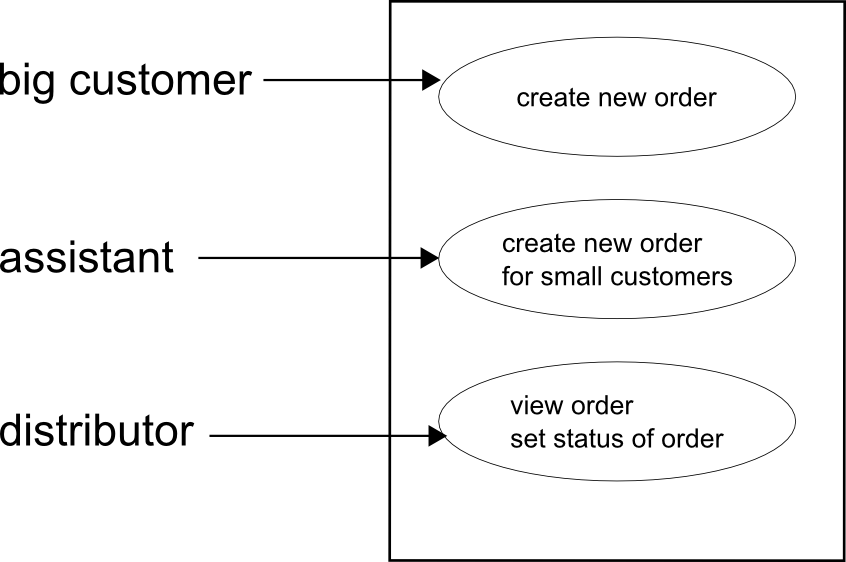
\includegraphics[scale=0.8]{../pics/umweltdiagramm.png}
 \end{center}
 \caption{The environmental view of the product}
\end{figure}


\chapter{Product Functionality}
\begin{tabbing}
    xxxxxxxxxx \= xxxxx \kill
    /LF10/ \> \textbf{Process:} search for a book\\
	\> \textbf{Actor:} customer\\ 
	\>\textbf{Description:} If a customer wants to order a book, he first has to search for it. A book can be searched by ISBN, title, author, year of publishing and genre.\\
	
	/LF20/ \> \textbf{Process:} modify order card\\
	\> \textbf{Actor:} customer\\ 
	\>\textbf{Description:} It should be possible to have all items on an order card. A person can add or delete books to that card.\\
\end{tabbing}

\chapter{Product Specification}
\chapter{Product Performance}
\chapter{Quality Requirements}
\begin{table}[h!]
 \begin{tabular}{lllll}
  \hline
  Quality & very good & good & normal & irrelevant \\
  \hline
  Functionality & X & & & \\
  Reliability & X & & & \\
  Usability & & & X & \\
  Efficiency & & X & & \\
  Modifiability & & & X & \\
  Portability & & & & X \\
  \hline
 \end{tabular}
\end{table}

\chapter{Additions}
None.

\end{document}